\section{Sicherheitsvollständige Testsuite}
\begin{frame}
\frametitle{Safety-related Output Abstraction}
\begin{itemize}
  \item<1-> Reaktion des Systems wird durch DFSM-Ausgabe modelliert
  \item<2-> Idee: Falsche Ausgabe muss nicht sicherheitsrelevant sein
  \item<3-> Sicherheitskritische Reaktionen definieren
  \item<4-> Nicht-sicherheitskritische Reaktionen zusammenfassen
\end{itemize}
\end{frame}

\begin{frame}
\frametitle{safety-Äquivalenz}
\begin{itemize}
  \item<1-> \emph{safety related output abstraction}: $\leq_s \subseteq \Sigma_O \times \Sigma_O$
  \item<2-> $\leq_s$ sei reflexiv, transitiv.
  \item<3-> s-äquivalent: $y_1 \sim_s y_2 \equiv y_1 \leq_s y_2$ und $y_2 \leq_s y_1$
  \item<4-> Zwei I/O-Folgen $X/Y, X'/Y'$ sind s-äquivalent gdw. $X=X'$ und $Y$ und $Y'$ sind s-äquivalent
  \item<5-> Zwei Zustände $q, q'$ sind s-äquivalent gdw. die Outputs für jede Inputfolge s-äquivalent sind.
  \item<6-> Zwei Systeme sind s-äquivalent gdw. ihre Anfangszustände s-äquivalent sind.
\end{itemize}
\end{frame}

\begin{frame}
\frametitle{Safety-Complete Test Suite}
Eine Test Suite $TS$ wird \emph{safety complete} genannt, gdw. für jede IUT $M'$ der Fehlerdomain gilt:
\begin{itemize}
  \item<1-> Soundness: $M$ und $M'$ sind I/O-äquivalent zueinander $\Rightarrow$ $M'$ besteht die Teset Suite ($M'~ \underline{pass}~ TS$)
  \item<2-> safety-Exhaustiveness: Für alle $M'$ aus der Fehlerdomain gilt: $M' \not \sim_s M \Rightarrow M'~ \underline{fail}~ TS$
\end{itemize}
\end{frame}

\begin{frame}
\frametitle{Beispiel}
\begin{columns}[T] % align columns

\begin{column}{.50\textwidth}
\textbf{M}
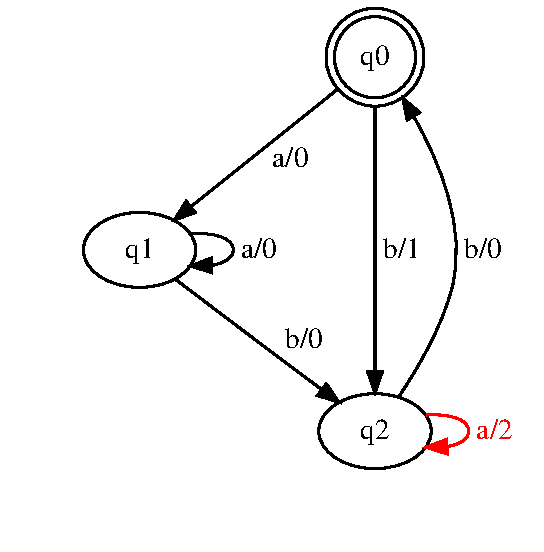
\includegraphics[width=\textwidth]{images/fsm-example01}
\end{column}%

\begin{column}{.50\textwidth}
\textbf{Safety Abstraktion von M}\\
\begin{itemize}
\item Ausgaben $0,1$  $\rightarrow Y$
\item Ausgabe $2$ ist safety-relevant: unverändert lassen
\end{itemize}
\end{column}%
\end{columns}
\end{frame}



\begin{frame}
\frametitle{Beispiel}
\begin{columns}[T] % align columns

\begin{column}{.50\textwidth}
\textbf{M}
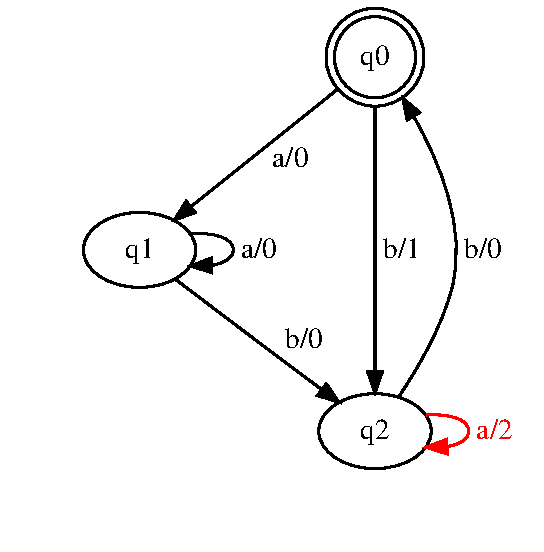
\includegraphics[width=\textwidth]{images/fsm-example01}
\end{column}%

\begin{column}{.50\textwidth}
\textbf{Safety Abstraktion von M}
\only<1>{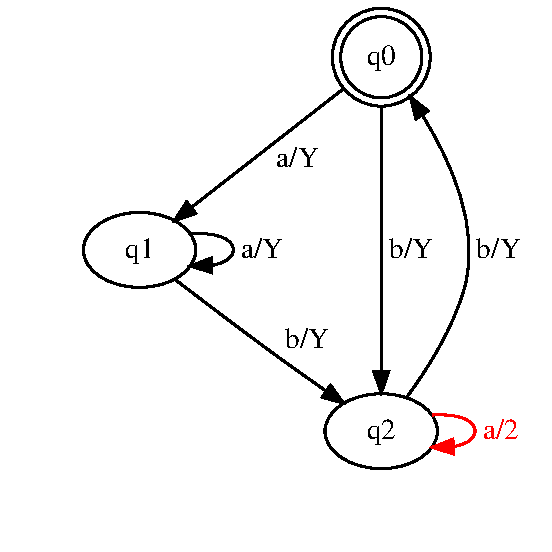
\includegraphics[width=\textwidth]{images/fsm-example01_abs}}%
\only<2->{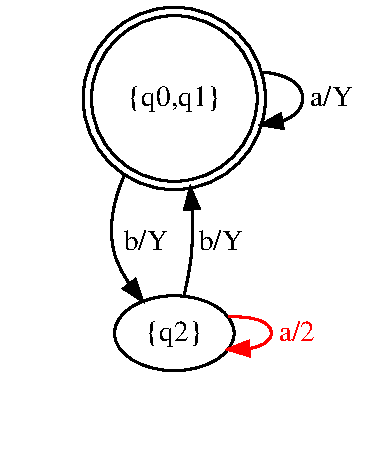
\includegraphics[width=0.8\textwidth]{images/fsm-example01_abs_min}}%
\end{column}%
\end{columns}
\end{frame}